\documentclass{standalone}
\usepackage{pgfplots}
\pgfplotsset{compat=1.11}
\begin{document}
% Place the TikZ picture in a figure environment.
%\begin{figure}[htb]
% h: here, t: top, b: bottom, p: page of float
%% https://tex.stackexchange.com/questions/39017/how-to-influence-the-position-of-float-environments-like-figure-and-table-in-lat
%% ! indicates that some restrictions should be ignored (discussed later)
%% h indicates that the float is allowed to be placed inline
%% t indicates that the float is allowed to go into a top area
%% b indicates that the float is allowed to go into a bottom area
%% p indicates the the float is allowed to go on a float page or column area

    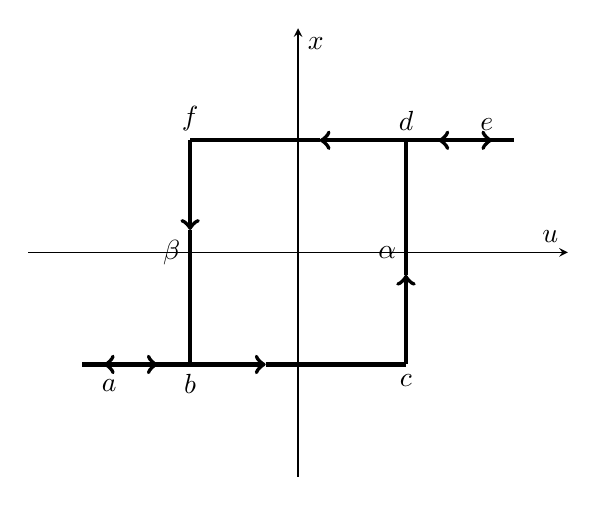
\begin{tikzpicture}
        \begin{axis} [
            xmin=-2.5, xmax=2.5, ymin=-2, ymax=2, 
            % grid=both,
            ylabel={$x$}, xlabel={$u$},
            % xtick={-2,-1.5,...,2}, ytick={-2,-1.5,...,2},
            % xticklabel style={font=\tiny, xshift=0.5ex},
            % yticklabel style={font=\tiny, yshift=0.5ex},
            axis line style={->},
            axis x line=middle,
            axis y line=middle,
            ticks=none
        ]
        \addplot+[line width=1.5pt, color=black, dashed, ->, mark=none, domain=-1.3:-1.8] {-1};
        \addplot+[line width=1.5pt,color=black, solid, ->, mark=none, domain=-2:-1.3] {-1};
        \addplot+[line width=1.5pt,color=black, solid, ->, mark=none, domain=-2:-0.3] {-1};
        \addplot+[line width=1.5pt,color=black, solid, mark=none, domain=-0.3:1] {-1};

        \addplot+[line width=1.5pt,color=black, solid, mark=none, ->,domain=1.3:1.8] {+1};

        \addplot+[line width=1.5pt,color=black, solid, mark=none, ->,domain=2:1.3] {+1};
        \addplot+[line width=1.5pt,color=black, solid, mark=none, ->, domain=1.3:0.2] {+1};
        \addplot+[line width=1.5pt,color=black, solid, mark=none, domain=0.2:-1] {+1};

        \draw[line width=1.5pt,color=black, solid, mark=none, ->] (1, -1) -- (1, -0.2);
        \draw[line width=1.5pt,color=black, solid, mark=none] (1, -0.2) -- (1, +1);

        \draw[line width=1.5pt,color=black, solid, mark=none, ->] (-1, +1) -- (-1, +0.2);
        \draw[line width=1.5pt,color=black, solid, mark=none] (-1, +0.2) -- (-1, -1);

        \node[below] at (-1.75,-1.05) {$a$};
        \node[below] at (-1,-1) {$b$};
        \node[below] at (1,-1) {$c$};
        \node[above] at (1,1) {$d$};
        \node[above] at (1.75,1) {$e$};

        \node[above] at (-1,1) {$f$};
        
        \node[left] at (-1,0) {$\beta$};
        \node[left] at (1,0) {$\alpha$};
        
        \end{axis}
    \end{tikzpicture}

\end{document}